%%==================================================================%%
%% Author : Tejedo Gonz�lez, Daniel                                 %%
%%          S�nchez Barreiro, Pablo                                 %%
%% Version: 1.0, 18/11/2012                                         %%
%% Version: 2.0, 06/02/2013                                         %%
%%                                                                  %%
%% Memoria del Proyecto Fin de Carrera                              %%
%% Antecedentes, emftext                                            %%
%%==================================================================%%


EMFText~\cite{emftext:2009} es una herramienta para dise�ar sintaxis textuales para metamodelos Ecore, siguiendo un enfoque de Ingenier�a de Lenguajes Dirigida por Modelos. Utilizando EMFText podemos definir la sintaxis textual de un lenguaje software utilizando una notaci�n similar a las de las notaci�n BNF. La Figura~\ref{fig:sle:gramaticaGrafos} muestra un ejemplo de gram�tica definida en EMFText para el lenguaje de grafos presentado en la Secci�n~\ref{sec:intr:sle}. 

%%==================================================================%%
%% NOTA(Pablo): Aqu� haz una gram�tica en EMFText para el lenguaje  %%
%%              de grafos del Cap�tulo 1                            %%
%%==================================================================%%

\begin{figure}[!tb]
    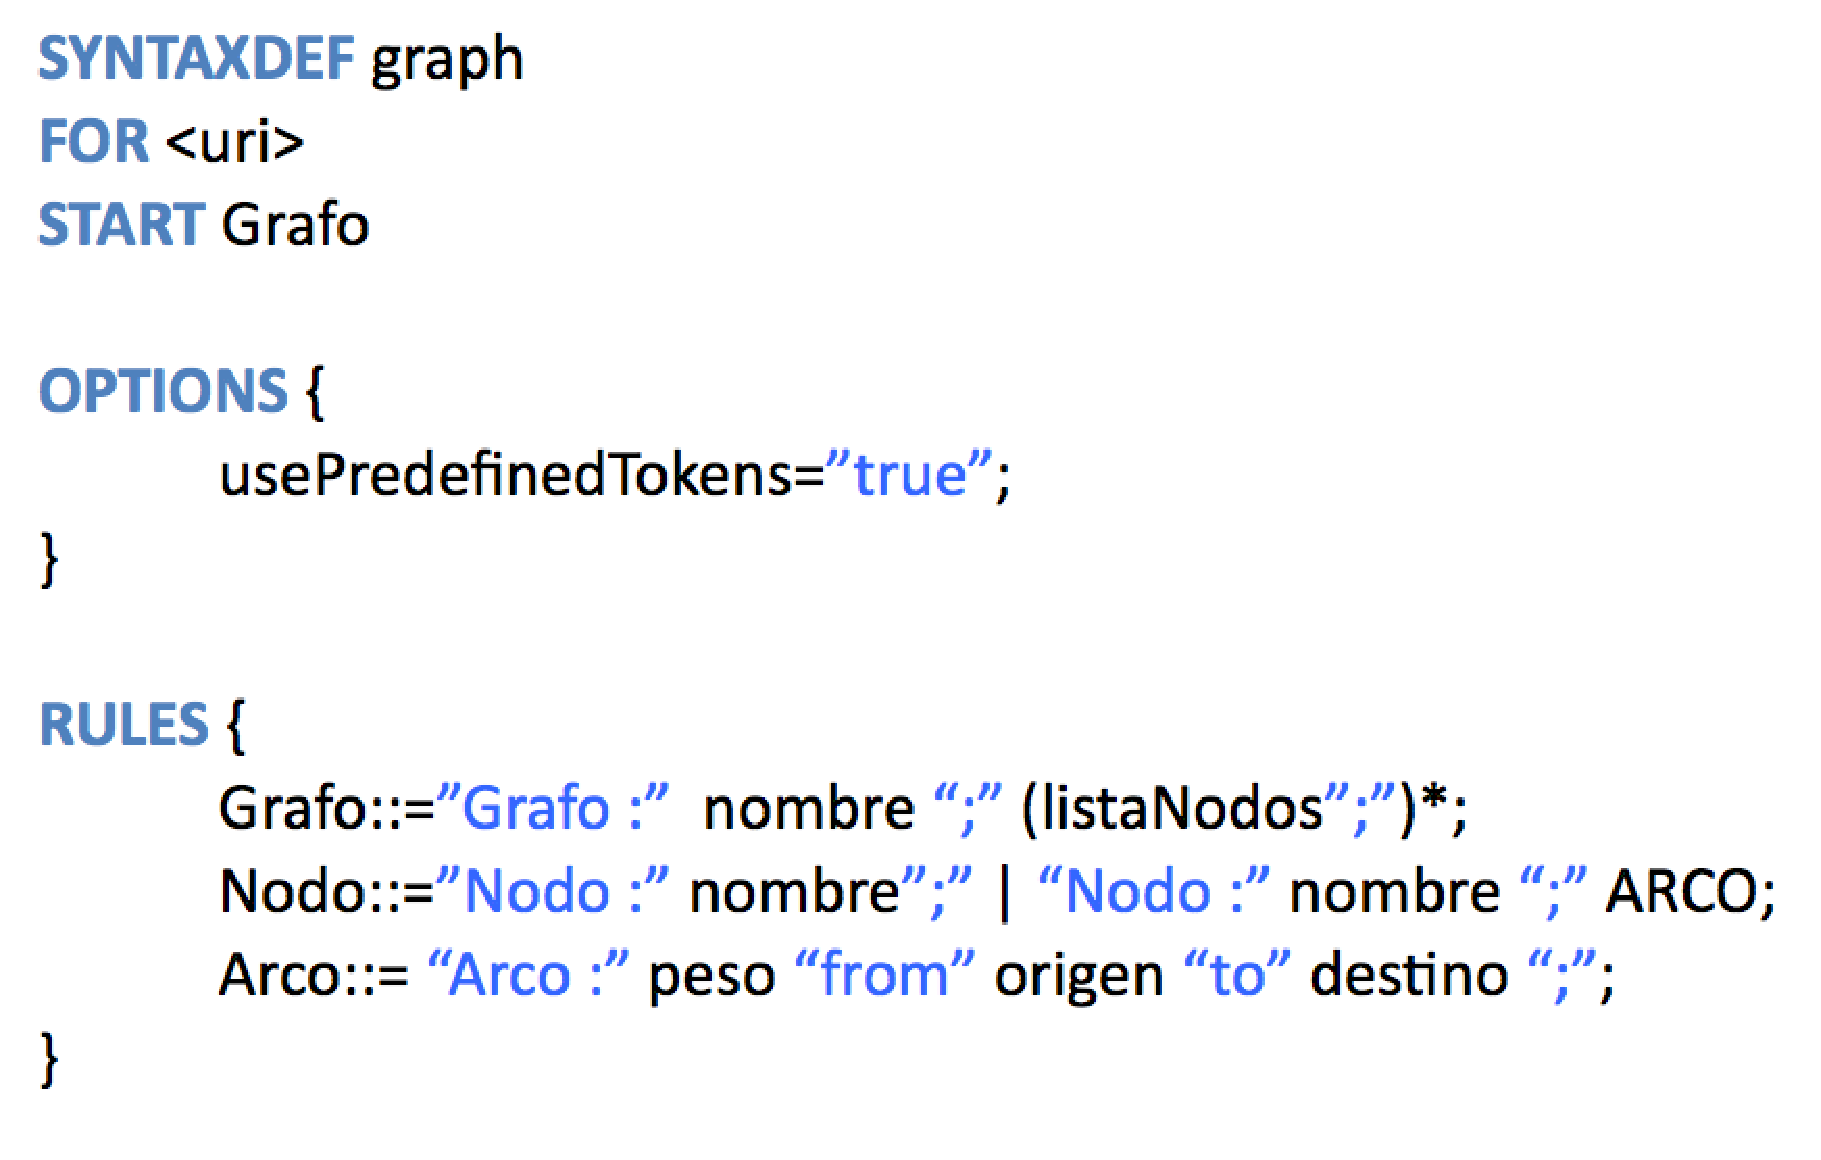
\includegraphics[scale=0.25]{background/gramaticaGrafo.eps}
    \caption{Gram�tica para el ejemplo del lenguaje de los grafos}
    \label{fig:sle:gramaticaGrafos}
\end{figure}

La sintaxis de EMFText difiere de las sintaxis BNF en que existen una serie de directivas para asociar elementos de la sintaxis textual con metaclases, de forma que se generen instancias de dichas metaclases a medida que se procesa el c�digo de un modelo. Por ejemplo, tal y como est� definida la gram�tica de la Figura~\ref{fig:sle:gramaticaGrafos}, a medida que vamos definiendo los arcos estamos indicando la informaci�n tanto de su peso como de sus nodos origen y destino. De este modo, EMFText genera una instanciaci�n de la metaclase Arco que inicializa con los datos le�dos y la a�ade a la instancia global del metamodelo.

La gran ventaja de EMFText es que permite generar, a partir de la definici�n de una gram�tica, una gran cantidad de c�digo, liberando al programador de tareas tediosas que adem�s en muchos casos podr�an resultar complicadas. Utilizando EMFText se puede generar autom�ticamente: (1) un editor para nuestro lenguaje, con facilidades como coloreado de la sintaxis o autocompletado; (2) un procesador para el lenguaje capaz de generar una instancia de su correspondiente metamodelo; y (3) el c�digo necesario para empaquetar y distribuir dicho editor como un \emph{plug-in} para Eclipse. Adem�s, todo el c�digo generado es completamente independiente de EMFText, por lo que puede ser ejecutado en plataformas que no tengan instalado dicha herramienta; y es personalizable. Por ejemplo, se puede modificar f�cilmente el postprocesador de nuestra gram�tica. 




